\documentclass[tikz,border=10pt]{standalone}
\usepackage{tikz}
\usetikzlibrary{shapes,arrows.meta,positioning,calc,decorations.pathmorphing}

\begin{document}

% Figure 1: Bernoulli Type Hierarchy
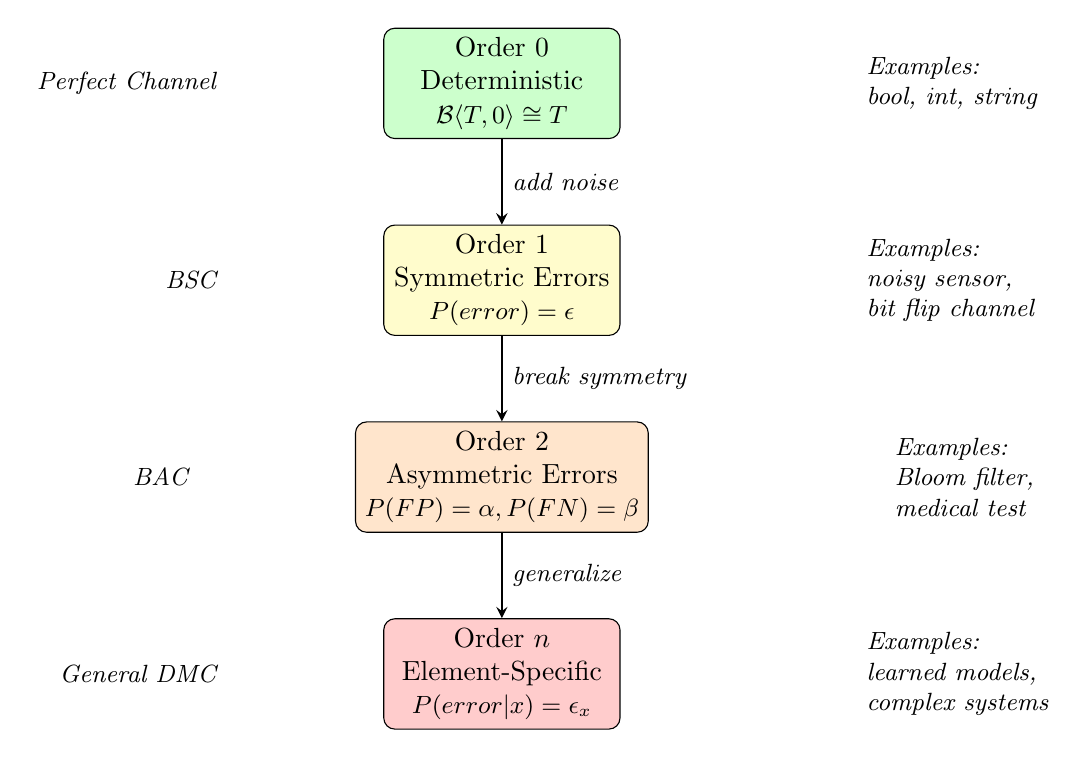
\begin{tikzpicture}[
    box/.style={draw, rectangle, rounded corners, minimum width=3cm, minimum height=1cm, align=center},
    exact/.style={box, fill=green!20},
    approx1/.style={box, fill=yellow!20},
    approx2/.style={box, fill=orange!20},
    approxn/.style={box, fill=red!20},
    arrow/.style={->, >=stealth, thick},
    label/.style={font=\small\itshape}
]

% Nodes
\node[exact] (order0) at (0,0) {Order 0\\Deterministic\\{\small $\mathcal{B}\langle T, 0 \rangle \cong T$}};
\node[approx1] (order1) at (0,-2.5) {Order 1\\Symmetric Errors\\{\small $P(error) = \epsilon$}};
\node[approx2] (order2) at (0,-5) {Order 2\\Asymmetric Errors\\{\small $P(FP) = \alpha, P(FN) = \beta$}};
\node[approxn] (ordern) at (0,-7.5) {Order $n$\\Element-Specific\\{\small $P(error|x) = \epsilon_x$}};

% Arrows
\draw[arrow] (order0) -- (order1) node[midway, right, label] {add noise};
\draw[arrow] (order1) -- (order2) node[midway, right, label] {break symmetry};
\draw[arrow] (order2) -- (ordern) node[midway, right, label] {generalize};

% Side annotations
\node[left=2cm of order0, label] {Perfect Channel};
\node[left=2cm of order1, label] {BSC};
\node[left=2cm of order2, label] {BAC};
\node[left=2cm of ordern, label] {General DMC};

% Examples on the right
\node[right=3cm of order0, align=left, label] {Examples:\\bool, int, string};
\node[right=3cm of order1, align=left, label] {Examples:\\noisy sensor,\\bit flip channel};
\node[right=3cm of order2, align=left, label] {Examples:\\Bloom filter,\\medical test};
\node[right=3cm of ordern, align=left, label] {Examples:\\learned models,\\complex systems};

\end{tikzpicture}

% Figure 2: Error Propagation in Composition
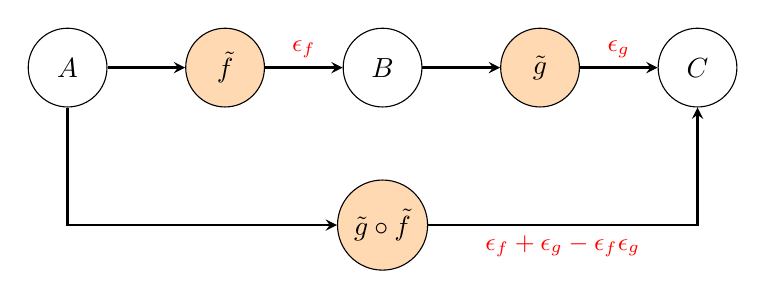
\begin{tikzpicture}[
    func/.style={draw, circle, minimum size=1cm},
    bernoulli/.style={func, fill=orange!30},
    arrow/.style={->, >=stealth, thick},
    error/.style={font=\small, text=red}
]

% Function composition
\node[func] (A) at (0,0) {$A$};
\node[bernoulli] (f) at (2,0) {$\tilde{f}$};
\node[func] (B) at (4,0) {$B$};
\node[bernoulli] (g) at (6,0) {$\tilde{g}$};
\node[func] (C) at (8,0) {$C$};

% Arrows
\draw[arrow] (A) -- (f);
\draw[arrow] (f) -- (B) node[midway, above, error] {$\epsilon_f$};
\draw[arrow] (B) -- (g);
\draw[arrow] (g) -- (C) node[midway, above, error] {$\epsilon_g$};

% Composed function
\node[bernoulli] (comp) at (4,-2) {$\tilde{g} \circ \tilde{f}$};
\draw[arrow] (A) |- (comp);
\draw[arrow] (comp) -| (C) node[near start, below, error] {$\epsilon_f + \epsilon_g - \epsilon_f \epsilon_g$};

\end{tikzpicture}

% Figure 3: Bernoulli Boolean Channel Model
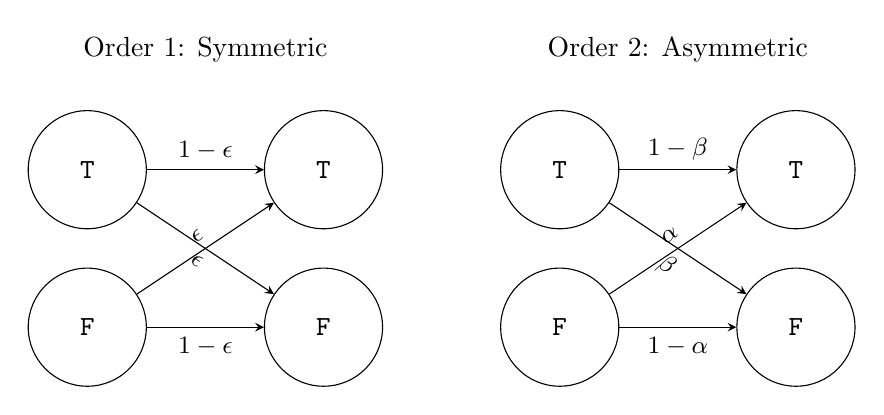
\begin{tikzpicture}[
    state/.style={draw, circle, minimum size=1.5cm},
    arrow/.style={->, >=stealth},
    prob/.style={font=\small}
]

% Order 1: Symmetric
\begin{scope}[local bounding box=symmetric]
\node[state] (T1) at (0,1) {$\mathtt{T}$};
\node[state] (F1) at (0,-1) {$\mathtt{F}$};
\node[state] (T1out) at (3,1) {$\mathtt{T}$};
\node[state] (F1out) at (3,-1) {$\mathtt{F}$};

\draw[arrow] (T1) -- (T1out) node[midway, above, prob] {$1-\epsilon$};
\draw[arrow] (T1) -- (F1out) node[midway, below, prob, sloped] {$\epsilon$};
\draw[arrow] (F1) -- (F1out) node[midway, below, prob] {$1-\epsilon$};
\draw[arrow] (F1) -- (T1out) node[midway, above, prob, sloped] {$\epsilon$};

\node[above=0.5cm of symmetric] {Order 1: Symmetric};
\end{scope}

% Order 2: Asymmetric
\begin{scope}[xshift=6cm, local bounding box=asymmetric]
\node[state] (T2) at (0,1) {$\mathtt{T}$};
\node[state] (F2) at (0,-1) {$\mathtt{F}$};
\node[state] (T2out) at (3,1) {$\mathtt{T}$};
\node[state] (F2out) at (3,-1) {$\mathtt{F}$};

\draw[arrow] (T2) -- (T2out) node[midway, above, prob] {$1-\beta$};
\draw[arrow] (T2) -- (F2out) node[midway, below, prob, sloped] {$\beta$};
\draw[arrow] (F2) -- (F2out) node[midway, below, prob] {$1-\alpha$};
\draw[arrow] (F2) -- (T2out) node[midway, above, prob, sloped] {$\alpha$};

\node[above=0.5cm of asymmetric] {Order 2: Asymmetric};
\end{scope}

\end{tikzpicture}

% Figure 4: Set Operations Error Propagation
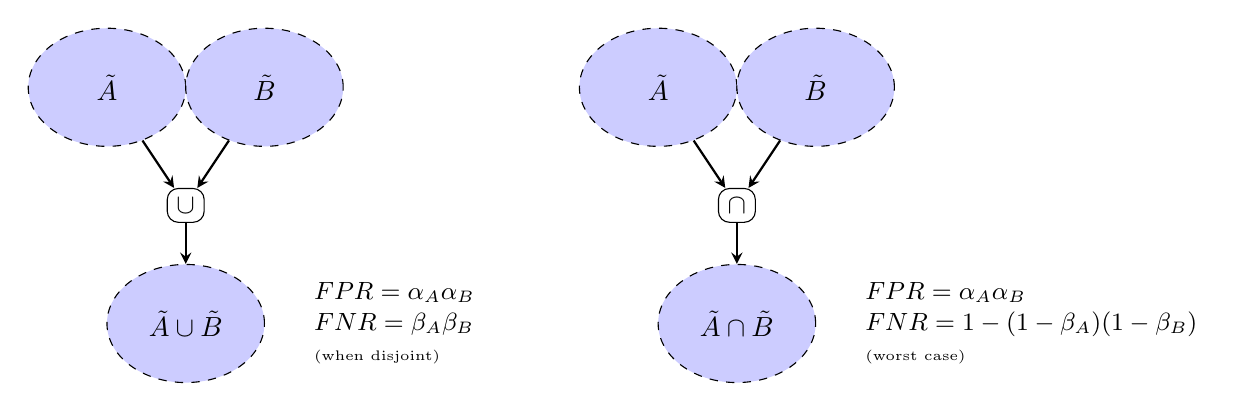
\begin{tikzpicture}[
    set/.style={draw, ellipse, minimum width=2cm, minimum height=1.5cm},
    bernoulli/.style={set, fill=blue!20, dashed},
    op/.style={draw, rectangle, rounded corners},
    arrow/.style={->, >=stealth, thick}
]

% Union operation
\begin{scope}[local bounding box=union]
\node[bernoulli] (A1) at (0,0) {$\tilde{A}$};
\node[bernoulli] (B1) at (2,0) {$\tilde{B}$};
\node[op] (union) at (1,-1.5) {$\cup$};
\node[bernoulli] (result1) at (1,-3) {$\tilde{A} \cup \tilde{B}$};

\draw[arrow] (A1) -- (union);
\draw[arrow] (B1) -- (union);
\draw[arrow] (union) -- (result1);

\node[right=0.5cm of result1, align=left, font=\small] {
    $\text{FPR} = \alpha_A \alpha_B$\\
    $\text{FNR} = \beta_A \beta_B$\\
    {\tiny (when disjoint)}
};
\end{scope}

% Intersection operation
\begin{scope}[xshift=7cm, local bounding box=intersection]
\node[bernoulli] (A2) at (0,0) {$\tilde{A}$};
\node[bernoulli] (B2) at (2,0) {$\tilde{B}$};
\node[op] (intersect) at (1,-1.5) {$\cap$};
\node[bernoulli] (result2) at (1,-3) {$\tilde{A} \cap \tilde{B}$};

\draw[arrow] (A2) -- (intersect);
\draw[arrow] (B2) -- (intersect);
\draw[arrow] (intersect) -- (result2);

\node[right=0.5cm of result2, align=left, font=\small] {
    $\text{FPR} = \alpha_A \alpha_B$\\
    $\text{FNR} = 1-(1-\beta_A)(1-\beta_B)$\\
    {\tiny (worst case)}
};
\end{scope}

\end{tikzpicture}

% Figure 5: Bernoulli Type Monad Structure
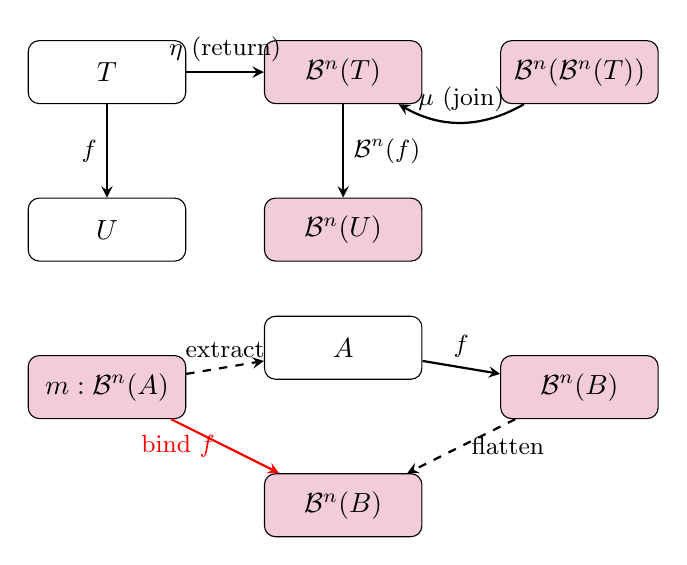
\begin{tikzpicture}[
    type/.style={draw, rectangle, rounded corners, minimum width=2cm, minimum height=0.8cm},
    monad/.style={type, fill=purple!20},
    arrow/.style={->, >=stealth, thick},
    label/.style={font=\small}
]

% Basic monad operations
\node[type] (T) at (0,0) {$T$};
\node[monad] (BT) at (3,0) {$\mathcal{B}^n(T)$};
\node[monad] (BBT) at (6,0) {$\mathcal{B}^n(\mathcal{B}^n(T))$};

% Return (eta)
\draw[arrow] (T) -- (BT) node[midway, above, label] {$\eta$ (return)};

% Join (mu)
\draw[arrow, bend left=30] (BBT) to node[above, label] {$\mu$ (join)} (BT);

% Fmap
\node[type] (U) at (0,-2) {$U$};
\node[monad] (BU) at (3,-2) {$\mathcal{B}^n(U)$};
\draw[arrow] (T) -- (U) node[midway, left, label] {$f$};
\draw[arrow] (BT) -- (BU) node[midway, right, label] {$\mathcal{B}^n(f)$};

% Bind operation visualization
\begin{scope}[yshift=-4cm]
\node[monad] (ma) at (0,0) {$m : \mathcal{B}^n(A)$};
\node[type] (a) at (3,0.5) {$A$};
\node[monad] (mb) at (6,0) {$\mathcal{B}^n(B)$};
\node[monad] (result) at (3,-1.5) {$\mathcal{B}^n(B)$};

\draw[arrow, dashed] (ma) -- (a) node[midway, above, label] {extract};
\draw[arrow] (a) -- (mb) node[midway, above, label] {$f$};
\draw[arrow, dashed] (mb) -- (result) node[midway, right, label] {flatten};
\draw[arrow, thick, red] (ma) -- (result) node[midway, left, label] {bind $f$};
\end{scope}

\end{tikzpicture}

\end{document}